% Exam Template for UMTYMP and Math Department courses
%
% Using Philip Hirschhorn's exam.cls: http://www-math.mit.edu/~psh/#ExamCls
%
% run pdflatex on a finished exam at least three times to do the grading table on front page.
%
%%%%%%%%%%%%%%%%%%%%%%%%%%%%%%%%%%%%%%%%%%%%%%%%%%%%%%%%%%%%%%%%%%%%%%%%%%%%%%%%%%%%%%%%%%%%%%

% These lines can probably stay unchanged, although you can remove the last
% two packages if you're not making pictures with tikz.
\documentclass[11pt]{exam}
\RequirePackage{amssymb, amsfonts, amsmath, latexsym, verbatim, xspace, setspace}
\RequirePackage{tikz, pgflibraryplotmarks}

%Path relative to the main .tex file 
\graphicspath{ {./img/} }

% By default LaTeX uses large margins.  This doesn't work well on exams; problems
% end up in the "middle" of the page, reducing the amount of space for students
% to work on them.
\usepackage[margin=1in]{geometry}
\usepackage{changepage}


% Here's where you edit the Class, Exam, Date, etc.
\newcommand{\class}{ICS 143A}
\newcommand{\term}{Fall 2017}
\newcommand{\examnum}{Midterm}
\newcommand{\examdate}{11/15/2017}
\newcommand{\timelimit}{9:00am - 9:50am}

% For an exam, single spacing is most appropriate
\singlespacing
% \onehalfspacing
% \doublespacing

% For an exam, we generally want to turn off paragraph indentation
\parindent 0ex

\begin{document} 

% These commands set up the running header on the top of the exam pages
\pagestyle{head}
\firstpageheader{}{}{}
\runningheader{\class}{\examnum\ - Page \thepage\ of \numpages}{\examdate}
\runningheadrule

\begin{flushright}
\begin{tabular}{p{2.8in} r l}
\textbf{\class} & \textbf{Name (Print):} & \makebox[2in]{\hrulefill}\\
\textbf{\term} &&\\
\textbf{\examnum} &&\\
\textbf{\examdate} &&\\
\textbf{Time Limit: \timelimit} & & \\
\end{tabular}\\
\end{flushright}
\rule[1ex]{\textwidth}{.1pt}




%\begin{minipage}[t]{3.7in}
%\vspace{0pt}
\begin{itemize}

\item \textbf{Don't forget to write your name on this exam.} 

\item \textbf{This is an open book, open notes exam. But no online or 
    in-class chatting.  } 

    
\item \textbf{Ask us if you something is confusing in the questions.}

\item \textbf{Organize your work}, in a reasonably neat and coherent way, in
the space provided. Work scattered all over the page without a clear ordering will 
receive very little credit.  

\item \textbf{Mysterious or unsupported answers will not receive full
credit}.  A correct answer, unsupported by explanation will receive no credit; 
an incorrect answer supported by substantially correct explanations might still 
receive partial credit.

\item If you need more space, use the back of the pages; clearly indicate when you have done this.
\end{itemize}

%Do not write in the table to the right.
%\end{minipage}
%\hfill

%\begin{minipage}[t]{2.3in}
%\vspace{0pt}
%\cellwidth{3em}
%\gradetablestretch{2}
\vqword{Problem}
\addpoints % required here by exam.cls, even though questions haven't started yet.	
\gradetable[v]%[pages]  % Use [pages] to have grading table by page instead of question

%\end{minipage}
\newpage % End of cover page

%%%%%%%%%%%%%%%%%%%%%%%%%%%%%%%%%%%%%%%%%%%%%%%%%%%%%%%%%%%%%%%%%%%%%%%%%%%%%%%%%%%%%
%
% See http://www-math.mit.edu/~psh/#ExamCls for full documentation, but the questions
% below give an idea of how to write questions [with parts] and have the points
% tracked automatically on the cover page.
%
%
%%%%%%%%%%%%%%%%%%%%%%%%%%%%%%%%%%%%%%%%%%%%%%%%%%%%%%%%%%%%%%%%%%%%%%%%%%%%%%%%%%%%%

\begin{questions}

% Basic question
\addpoints
\question Basic page tables.


\begin{parts}
\part[10] 

Illustrate the page table used by xv6 to map the kernel into the virtual
address space of each process (draw a page table diagram and explain the page
table entries). 
%
Specifically concentrate on one entry: the entry responsible for the
translation of the first page of the kernel code. 
%
Keep in mind that xv6 maps the kernel into the virtual address range starting
above the second gigabyte of virtual memory. 
%
Note, that after xv6 is done booting, it xv6 uses normal 4KB, 32bit, 2-level
page tables. 
%
You also have to recall the physical address of the first kernel page (look at
the boot lecture or the kernel map), and the virtual address where this page is
mapped. 
%
To make the example realistic, don't forget that xv6 allocates memory for it's
page table directory and page tables from the kernel memory allocator. 
%


\textbf{STUDENT SOLUTION } 
\begin{adjustwidth}{1.5em}{1em}
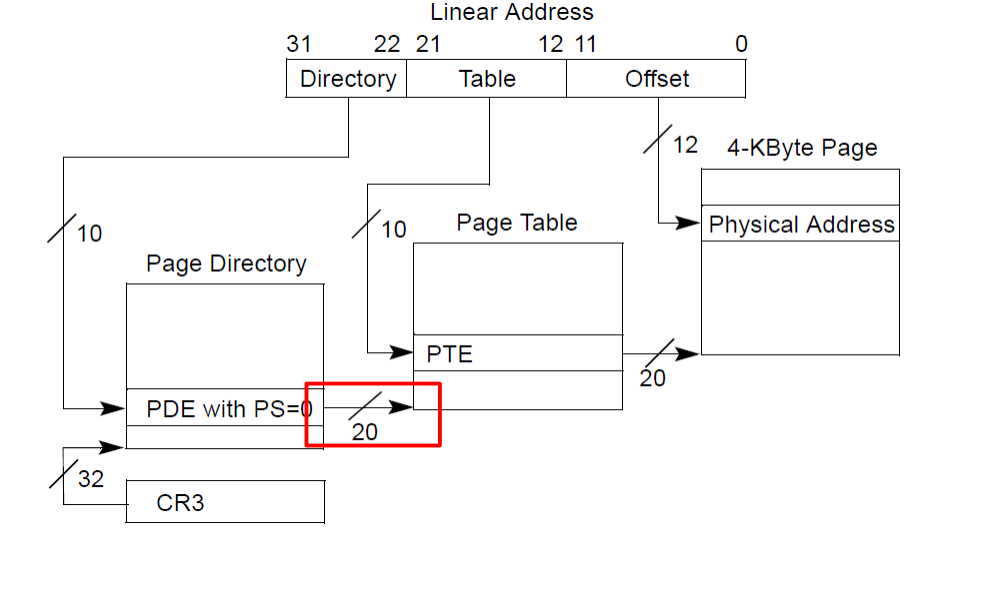
\includegraphics{paging}

The image above is a page table diagram used by xv6. For the first page of the kernel, 
 it is certainly at virtual address 0x80000000 (as is convention in xv6). 
We take its first 10 bits, and find out that this is at the 512th entry at the Page Table directory to 
find the location of the Page Table. 
Then we take the second 10 bits of the virtual address, which is 0 for the first page, 
and find the location of the Page Table Entry at the Page Table. Through the 0th entry 
of the Page table, we find out the physical address of the kernel, which should be at Physical 
address 0x00, and use the offset in the last 12 bits to find the physical address of the given 
memory address
\end{adjustwidth}

\vfill 


%\part[10] Imagine you want to construct a two-level page table but have only
%one 4K physical page for both page table directory, and all level 2 page
%tables. What kind of address spaces you will be able to consrtuct?  Draw a
%picture, provide some discussion.

\vfill
\end{parts} 

\newpage \addpoints

\question Alice works on implementing a new shell for xv6. She implements a
pipe command (e.g., ls $\vert$ wc) like this: 

\begin{verbatim} 
void
runcmd(struct cmd *cmd)
{
  ...
  switch(cmd->type){
  default:
    fprintf(stderr, "unknown runcmd\n");
    exit(-1);

  case '|': pcmd = (struct pipecmd*)cmd;
    int p[2];
    pipe(p);
    int pid = fork();
    if(pid == 0){
        //child process:left side
        close(1);
        dup(p[1]);
        close(p[1]);
        close(p[0]);
        runcmd(pcmd->left);
    }
    close(0);
    dup(p[0]);
    close(p[0]);
    close(p[1]);
    wait(NULL);
    runcmd(pcmd->right);
    break;
  } 
  ...  
} 
\end{verbatim}

\begin{parts} 

\part[5] Her implementation always waits for left side to finish, but she is
not sure if it's correct since she notices that the shell that xv6 implements
(sh.c in the xv6 source tree) launches the right side right away. Can you come
up with an example for which Alice's shell fails, while the xv6's is still
correct?  Explain your answer.
 

\textbf{STUDENT ANSWER} 
\begin{adjustwidth}{1.5em}{0pt}
In this version, the two ends of the pipe will execute sequentially. That is, the 
right end of the pipe will wait for the left end of the pipe to finish and exit and 
it will start to run. So suppose the left side take a long time to run, or the 
contents it puts into the pipe overloads the buffer and leads to a wait situation. 
In this situation, there will be an eternal wait as Alice's wait will never be triggered 
by the left cmd, as the left cmd's pipe is waiting for the pipe to be read from - 
which in turn will never be done as wait is never properly triggered, so the right 
side cannot read and free up buffer space for the left to contine executing creating 
a deadlock situation.
\end{adjustwidth}

\end{parts}

% Question with parts
\newpage
\addpoints 

\question OS isolation and protection

\begin{parts} 

\part[5] Explain the organization and memory layout of the xv6 process. Draw a
diagram. Explain which protection bits are set by the kernel and explain why
kernel does it.


\textbf{STUDENT ANSWER} 
\begin{adjustwidth}{1.5em}{0pt}
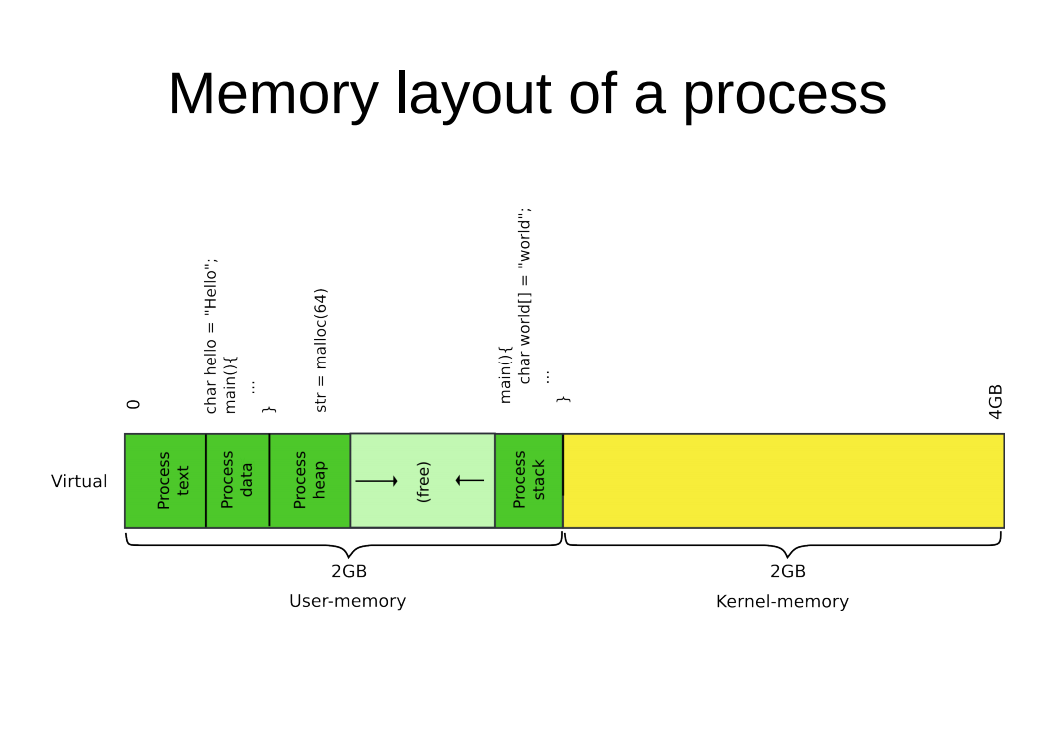
\includegraphics{memlayout}

Above is the organization of an xv6 process. Process Text holds code, Process Data holds variables and the like, 
Process Heap stores dynamically allocated variables, Guard Page (1 page between Heap and Stack) act as safe 
guard to overflow, and Process Stack is where variable calls/process stack/local variables are stored.

The main protection bit set by kernel is bit 2, which is U/S, the user supervisor bit. When 1, user may use, else 
only for kernel. This is done to allow for pages to be a general use memory segment, while providing protection 
for the kernel from user's modifying sensative data.
(see, intel volume 3a, table 4-19 on pg 131 of this pdf: 
https://software.intel.com/sites/default/files/managed/7c/f1/253668-sdm-vol-3a.pdf)

\end{adjustwidth}



\part[5] In xv6 individual processes are isolated, specifically they cannot
access each others memory. Explain how this is implemented. 


\textbf{STUDENT ANSWER} 
\begin{adjustwidth}{1.5em}{0pt}
Each process has its own page table. When reading from a virtual address, MMU 
will find physical address by reading this process's page table. The pages of other 
processes are not mapped to this process's page table, therefore, the physical 
address of other processes will never be the translate result of this process. 
\end{adjustwidth}

\vfill 

\iffalse

\newpage 

\part[10] Bob is very new to xv6, he writes his first program: 

\begin{verbatim}
#include "types.h"
#include "user.h"
  
int
main(int argc, char *argv[])
{   

  char buf[512], *p = 0;
    
  memmove(p, buf, sizeof(buf));
  exit();
}
\end{verbatim}

However, when he runs it, he gets the following error
\begin{verbatim}
$ copy
pid 3 copy: trap 14 err 5 on cpu 1 eip 0x0 addr 0x11f0--kill proc
$
\end{verbatim}

He notices that he initializes *p to 0x0, and explain what goes wrong. 

\fi


\end{parts} 

\newpage 

\addpoints

\question OS organization. 



\begin{parts} 


\part[10] \texttt{KERNBASE} limits the amount of memory a single process can
use, which might be irritating on a machine with a full 4 GB of RAM. Would
raising \texttt{KERNBASE} allow a process to use more memory (explain your answer)? 

\textbf{STUDENT ANSWER} 
\begin{adjustwidth}{1.5em}{0pt}
No. Raising KERNBASE will leave kernel space less memory. However, page table 
and mappings reside in the kernel space. Therefore, shrinking the space that a kernel 
can use will also shrink the space a user process can use. So this will not allow a process 
to use more memory.
\end{adjustwidth}
\vfill

\end{parts}

% If you want the total number of points for a question displayed at the top,
% as well as the number of points for each part, then you must turn off the
% point-counter or they will be double counted.
%\newpage
%\addpoints
%\question[10] Even more work.
%\noaddpoints % If you remove this line, the grading table will show 20 points 
%for this problem.
%\begin{parts} \part[5] Even more...  \vspace{4.5in} \part[5] That's clearly
%too much \end{parts}



\end{questions}
\end{document}
